\documentclass{siamart1116}
\usepackage{amsmath, amssymb}
%\usepackage{amsmath,amssymb,amsfonts,graphicx,amsthm,dsfont}
%\usepackage{listings}
%\usepackage{courier}
\usepackage{enumerate}
%\usepackage{color}
%\usepackage[usenames,dvipsnames]{xcolor}
%\usepackage{hyperref,tikz,mdframed}
%\hypersetup{colorlinks=true,urlcolor=MidnightBlue,citecolor=PineGreen,linkcolor=BrickRed}

% \lstset{
% 	basicstyle=\small\ttfamily,
% 	keywordstyle=\color{blue},
% 	language=python,
% 	xleftmargin=16pt,
% }
\usepackage{algorithmicx}
\usepackage{algpseudocode}% http://ctan.org/pkg/algorithmicx
\usepackage{multicol}

\textwidth=5.8in
\textheight=9in
\topmargin=-0.5in
\headheight=0in
\headsep=.5in
\hoffset  -.4in
\pagestyle{empty}

\newcommand{\Fp}{\mathbb{F}_p}
\newcommand{\Q}{\mathbb{Q}}
\newcommand{\Z}{\mathbb{Z}}
\newcommand{\kron}[2]{\left(\frac{#1}{#2}\right)}
\newcommand{\Aut}{\mathrm{Aut}}
\newcommand{\End}{\mathrm{End}}
\newcommand{\SO}{\mathrm{SO}}
\newcommand{\SU}{\mathrm{SU}}
\newcommand{\tr}{\operatorname{tr}}
\newcommand{\dee}{\mathrm{d}}
\newcommand{\deee}{\textbf{\text{\emph{d}}}}

\newcommand{\md}[1]{\textcolor{cyan}{#1}}

\newcommand{\TheAuthors}{V. Chen}

%\newtheorem{theorem}{Theorem}
%\newtheorem{definition}{Definition}

\graphicspath{ {graphics/} }

\title{Week 2 Summary}
\author{\TheAuthors}
\date{}
\begin{document}
\maketitle
\setlength{\unitlength}{1in}
\setlength{\parindent}{0in}

\section{Summary}
Last week's experiments indicated that the original parameterization, treating $u, \tau, \alpha$ as the variables, would not converge even after 100,000 iterations. First, we explain the different parameterization that we tried this week. We decided to try a different parameterization which treats $\xi, \tau, \alpha$ as variables to sample, and we compare results between this and the old parameterization.

\section{Learning $\tau$ and $\alpha$ with non-centered parameterization}
\subsection{Algorithm}
In the centered parameterization, the prior was $u|\tau,\alpha \sim N(0, C(\tau, \alpha))$, $\tau, \alpha$ distributed independently and uniformly over intervals. We would take the posterior by Bayes' theorem to be
\[f(u,\tau,\alpha) \propto \exp\left(-\Phi(u) -\frac{1}{2}\langle u, C(\tau,\alpha)^{-1}u \rangle - \frac{1}{2}\log(\det(C(\tau,\alpha))) + \log(\pi_0(\tau,\alpha))\right) \]
In the new parameterization, we sample $\xi \sim N(0, I)$ and $\tau, \alpha$ on uniform intervals as before. $\xi$ is related to $u$ by $T(\xi,\tau,\alpha) = u = \sum_{j=0}^{M}(\lambda_j+\tau^2)^{-\alpha/2}\xi_jq_j$. Recall that we are taking $M=N-1$. The new joint posterior becomes:
\[ g(\xi,\tau,\alpha) \propto \exp\left( -\Phi(T(\xi,\tau,\alpha))-\frac{1}{2}\langle u,u \rangle + \log(\pi_0(\tau,\alpha)) \right)\]
This algorithm works as follows:
\begin{algorithm}
\caption{Non-centered parameterization: sampling $\xi, \tau, \alpha$}
\label{alg:xi_tau_alpha}
\begin{algorithmic}
\State Choose $\xi^{(0)} \in \mathbb{R}^N, \alpha^{(0)}, \tau^{(0)} > 0, \beta \in (0, 1]$ and $\epsilon_1, \epsilon_2 > 0$.
\For{$k=0$ to $S$}
\State Propose $\hat\xi^{(k)} = (1-\beta^2)\xi^{(k)} + \beta \zeta^{(k)}$, $\zeta^{(k)} \sim N(0, I)$
\State Make transition $\xi^{(k+1)} \to \hat\xi^{(k)}$ with probability
\[ A(\xi^{(k)} \to \hat\xi^{(k)}) = \min\{1, \frac{g(\hat\xi^{(k)},\tau^{(k)},\alpha^{(k)})}{g(\xi^{(k)},\tau^{(k)},\alpha^{(k)})} \}\]

\State Propose $\hat\tau^{(k)} = \tau^{(k)} + \epsilon_1 \rho^{(k)}, \rho^{(k)} \sim N(0,I)$
\State Make transition $\tau^{(k+1)} \to \hat\tau^{(k)}$ with probability
\[ A(\tau^{(k)} \to \hat\tau^{(k)}) = \min\{1, \frac{g(\xi^{(k+1)},\hat\tau^{(k)},\alpha^{(k)})}{g(\xi^{(k+1)},\tau^{(k)},\alpha^{(k)})} \}\]

\State Propose $\hat\alpha^{(k)} = \alpha^{(k)} + \epsilon_2 \sigma^{(k)}, \sigma^{(k)} \sim N(0,I)$
\State Make transition $\alpha^{(k+1)} \to \hat\alpha^{(k)}$ with probability
\[ A(\alpha^{(k)} \to \hat\alpha^{(k)}) = \min\{1, \frac{g(\xi^{(k+1)},\tau^{(k+1)},\hat \alpha^{(k)})}{g(\xi^{(k+1)},\tau^{(k+1)},\alpha^{(k)})} \}\]
\EndFor
\State \Return $\{ T(\xi^{(k)},\tau^{(k)},\alpha^{(k)}), \tau^{(k)}, \alpha^{k} \}$
\end{algorithmic}
\end{algorithm}

\subsection{Simulation results}
The relevant figures are \cref{fig:hier_sim_1}, \cref{fig:hier_sim_2}, \cref{fig:hier_sim_3}, \cref{fig:hier_sim_4}, \cref{fig:hier_sim_5}, \cref{fig:hier_sim_6}. The parameters used are as follows:
\begin{center}
\begin{tabular}{| c | c |}
\hline
Iterations & 100000 \\ \hline
Burn in period & 1000 \\ \hline
Laplacian & self-tuning, unnormalized \\ \hline
$\beta$ & $0.1$\\ \hline
$\gamma$ & $0.0001$\\ \hline
Labeled +1 & $280-290$ \\ \hline
Labeled -1 & $20-30$ \\ \hline
$\epsilon_\alpha$ & $1$\\ \hline
$\epsilon_\tau$ & $1$\\ \hline
Initial $\tau$ & $30$\\ \hline
Initial $\alpha$ & $5$\\ \hline
$\tau$ range & $[0, 60]$\\ \hline
$\alpha$ range & $[0, 100]$\\ \hline
Average $\tau$ & $3.74$\\ \hline
Average $\alpha$ & $63.5$\\ \hline
Percent of correct classification & $0.864407$ \\ \hline
Time elapsed & 183.21 s \\ \hline
\end{tabular}
\end{center}

\begin{figure}[!htb]
    \begin{minipage}{0.48\textwidth}
        \centering
        \caption{\label{fig:hier_sim_1} $\alpha$ acceptance probability}
        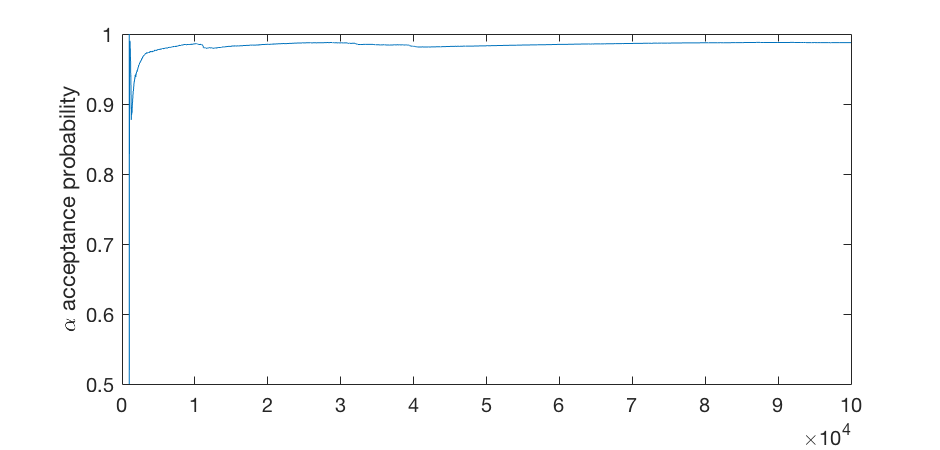
\includegraphics[width=\linewidth]{graphics/noncentered/acceptance_alpha_probability.png}
    \end{minipage} \hfill
    \begin{minipage}{0.48\textwidth}
        \centering
        \caption{\label{fig:hier_sim_2} $\alpha$ trace}
        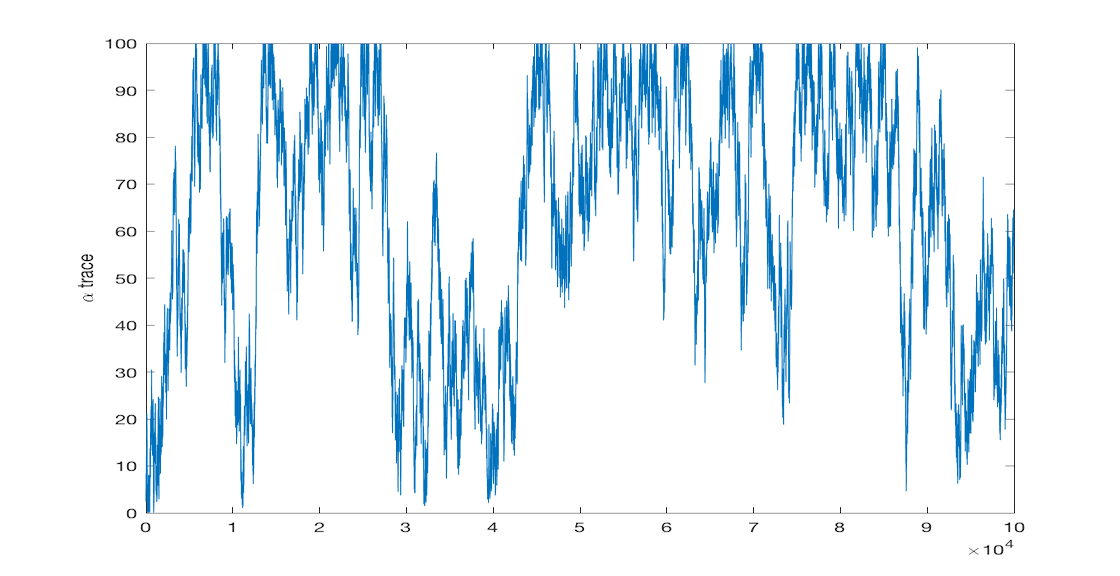
\includegraphics[width=\linewidth]{graphics/noncentered/trace_alpha.png}
    \end{minipage}
\end{figure}

\begin{figure}[!htb]
    \begin{minipage}{0.48\textwidth}
        \centering
        \caption{\label{fig:hier_sim_3} $\tau$ acceptance probability}
        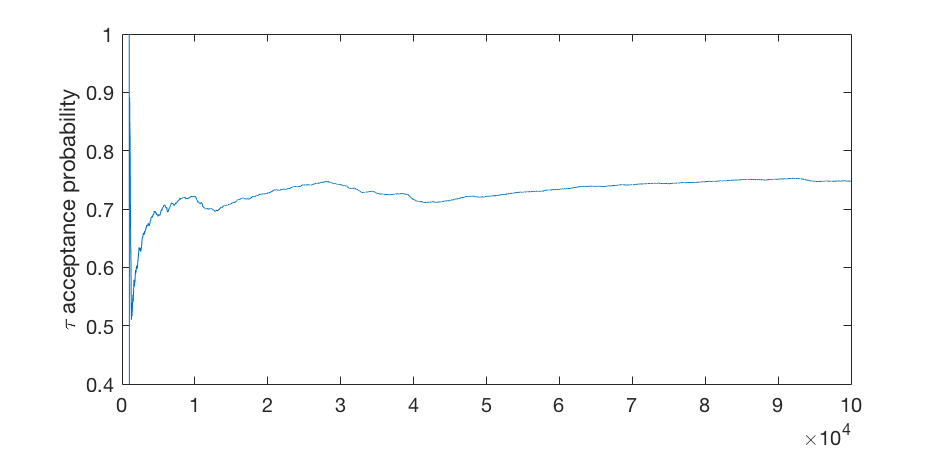
\includegraphics[width=\linewidth]{graphics/noncentered/acceptance_tau_probability.png}
    \end{minipage} \hfill
    \begin{minipage}{0.48\textwidth}
        \centering
        \caption{\label{fig:hier_sim_4}  $\tau$ trace}
        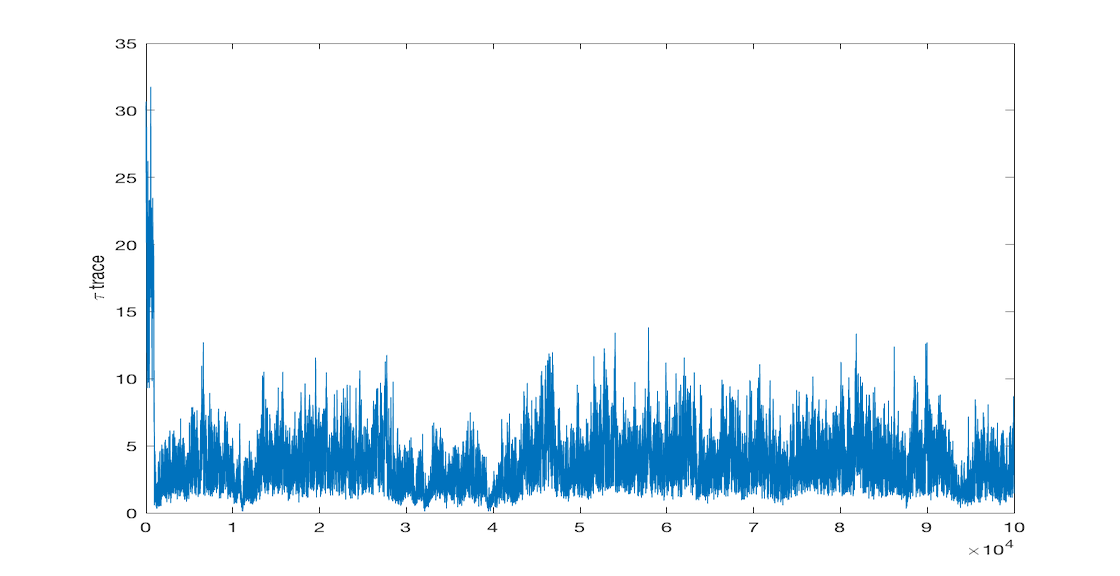
\includegraphics[width=\linewidth]{graphics/noncentered/trace_tau.png}
    \end{minipage}
\end{figure}

\begin{figure}[!htb]
    \begin{minipage}{0.48\textwidth}
        \centering
        \caption{\label{fig:hier_sim_5} $\xi$ acceptance probability}
        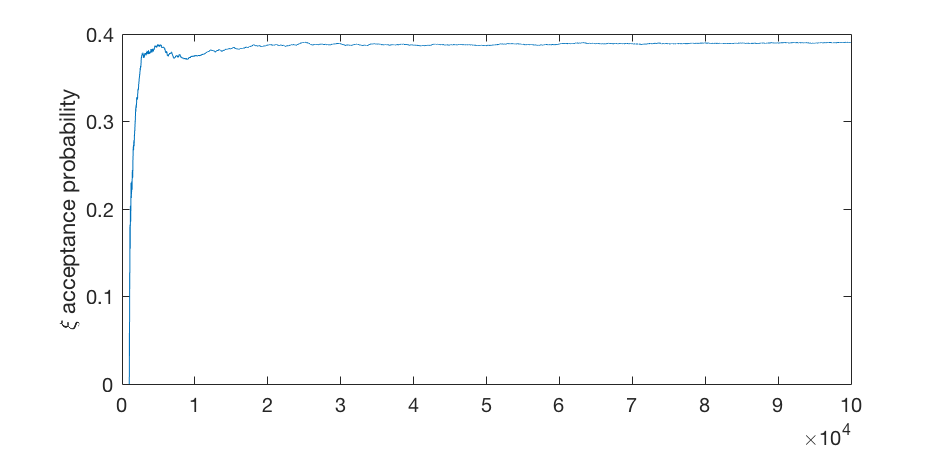
\includegraphics[width=\linewidth]{graphics/noncentered/acceptance_xi_probability.png}
    \end{minipage} \hfill
    \begin{minipage}{0.48\textwidth}
        \centering
        \caption{\label{fig:hier_sim_6} $u$ final average}
        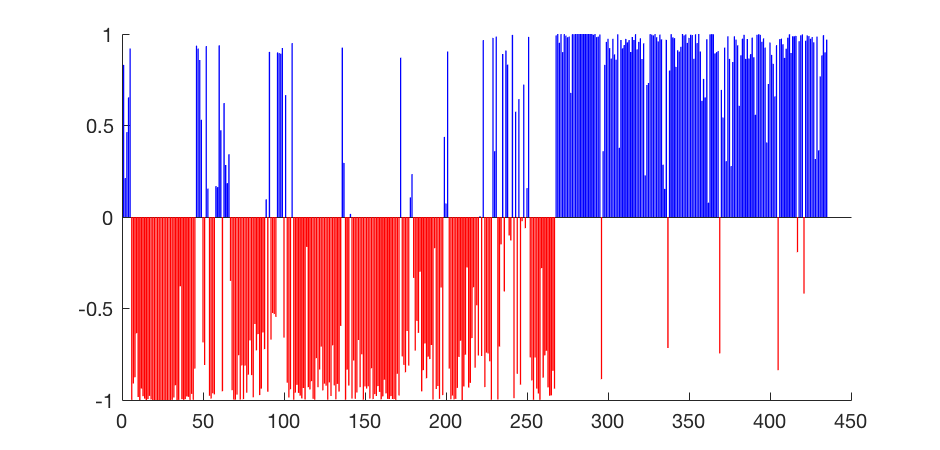
\includegraphics[width=\linewidth]{graphics/noncentered/final_avg.png}
    \end{minipage}
\end{figure}

\section{Revisiting the centered parameterization}

\section{Two moons data}
The non-centered parameterization with the unnormalized Laplacian does not perform well on the two moons data set. One possibility is that the first eigenvector in the unnormalized Laplacian is constant and is throwing off the classification. %insert figure?

Initializing from $u=0$ was also a bad idea because $\tau, \alpha$ would blow up to their max limit.
\end{document}